% !TEX program = xelatex
% 2026《人工智能导论》大作业报告
% 可解释谣言检测系统
\documentclass[10pt,conference]{IEEEtran}

% ===== 中文支持 =====
\usepackage{xeCJK}
\setCJKmainfont{SimSun}[AutoFakeBold=2.5]           % 正文：宋体
\setCJKsansfont{SimHei}[AutoFakeBold=2.5]            % 标题：黑体（section 用）
\setCJKmonofont{FangSong}                             % 等宽：仿宋（可选）

% 让 IEEEtran section 标题使用黑体
\usepackage{titlesec}
\titleformat{\section}{\centering\sffamily\large}{}{0em}{}
\titleformat{\subsection}{\sffamily\normalsize}{}{0em}{}

% ===== 基础包 =====
\usepackage{amsmath,amssymb,amsfonts}
\usepackage{graphicx}
\usepackage{xcolor}
\usepackage{hyperref}
\usepackage{url}
\usepackage{booktabs}
\usepackage{multirow}
\usepackage{float}

% 页面设置
\usepackage[letterpaper, margin=0.75in]{geometry}

% 超链接
\hypersetup{
    colorlinks=true,
    linkcolor=black,
    citecolor=blue,
    urlcolor=blue,
}

% 表格字体缩小
\newcommand{\tabfont}{\footnotesize}

\begin{document}

% ========================================
% 标题
% ========================================
\title{\textbf{可解释谣言检测系统}\\[2ex]
\large 基于 RoBERTa-large 分类与 DeepSeek-V3.2 解释的端到端框架}

\author{
\IEEEauthorblockN{韩宇飞、姜新晨、靳卓达}
\IEEEauthorblockA{上海交通大学 计算机学院\\
第六组\\
hanyufei24@sjtu.edu.cn}
}

\maketitle

% ========================================
% 1. 任务目标
% ========================================
\section{任务目标}

本大作业构建\textbf{可解释的谣言检测系统}：输入推文及事件 ID，输出二分类标签（谣言/非谣言）与判断依据的自然语言解释。数据集为英文推文，涵盖 7 个事件，训练集 2840 条，验证集 401 条。

% ========================================
% 2. 具体内容
% ========================================
\section{具体内容}

\subsection{实施方案}

系统采用\textbf{深度学习分类器 + 大语言模型解释器}的复合架构：

\begin{figure}[H]
\centering
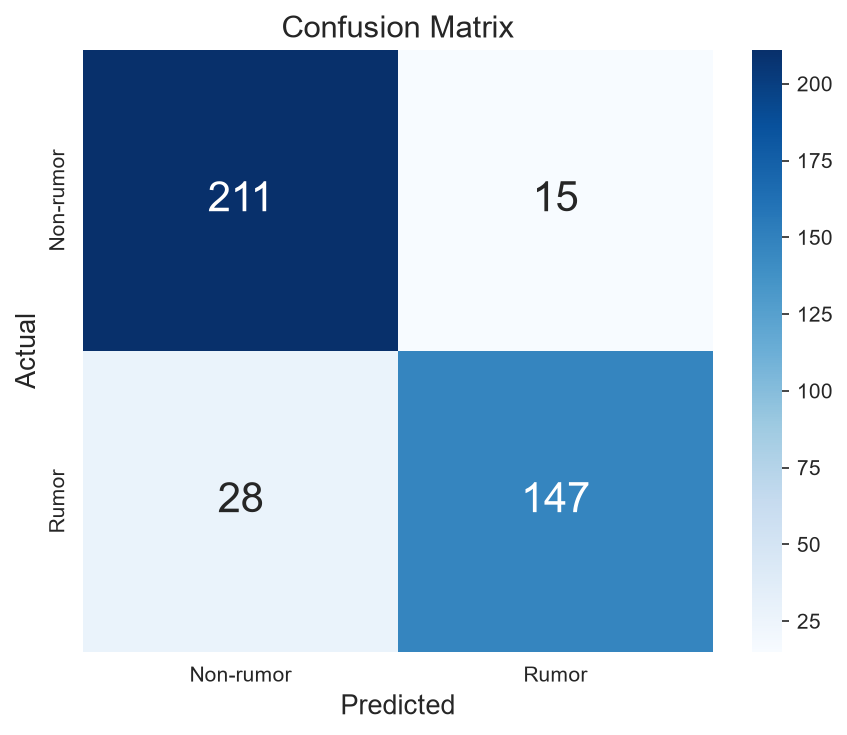
\includegraphics[width=0.85\columnwidth]{figures/confusion_matrix.png}
\caption{验证集混淆矩阵（401 条）}
\label{fig:cm}
\end{figure}

\textbf{分类器}：RoBERTa-large（355M）微调，验证集准确率 89.53\%。事件信息经 Embedding 层（7×32 维）与文本 [CLS] 拼接，避免传统 [EVENT\_N] token 与文本词的不必要交互。

\textbf{关键词提取}：末层多头注意力 [CLS] 分数平均后取 Top-5 词，作为判断线索。

\textbf{案例检索}：sentence-transformers 检索训练集中 Top-3 相似案例，供 LLM 参考。

\textbf{LLM 解释}：通过 SJTU API 调用 DeepSeek-V3.2，将文本、分类结果、关键词、相似案例、事件背景组装为 Prompt，生成中文解释。LLM 定位为透明解释者而非独立法官——实验表明独立法官会使准确率从 89\% 降至 65\%。

\textbf{置信度分级}：确信（$\ge$0.9）、倾向（0.7--0.9）、存疑（$<$0.7）三级，助用户识别不确定场景，低置信度样本输出复核提醒。

\subsection{核心代码分析}

系统采用模块化设计：

\textbf{models/classifier.py}：RumorClassifier 基于 HuggingFace AutoModel，支持 BERT/RoBERTa 系列。Event Embedding 与旧 token 模式兼容，load\_model() 统一加载。

\textbf{models/keyword\_extractor.py}：predict() 输出 \{label, confidence, keywords\}，兼容 BERT 与 RoBERTa 的 subword 合并。

\textbf{llm\_explainer.py}：LLMExplainer 封装 OpenAI 兼容 API 调用，含五要素 Prompt 构建与重试机制。

\textbf{inference.py}：端到端推理入口，--no-llm 约 4 分钟，完整模式约 39 分钟（API 限速）。

\textbf{adversarial.py}：一键对抗攻防评估，--mode compare 完成样本生成→推理→翻转率对比。

\subsection{检测结果分析}

\subsubsection{模型训练与超参搜索}

在 4×3090 GPU 上完成 15 组实验，搜索 BERT-base、RoBERTa-base、RoBERTa-large 三种架构：

\begin{table}[H]
\centering
\caption{最终模型在验证集（401 条）上的完整表现}
\label{tab:final}
\tabfont
\begin{tabular}{@{}lcc@{}}
\toprule
指标 & 数值 \\
\midrule
Accuracy & 89.53\% (359/401) \\
Precision & 90.30\% \\
Recall & 85.14\% \\
F1 Score & 87.65\% \\
FP（误报） & 16（4.0\%） \\
FN（漏报） & 26（6.5\%） \\
\bottomrule
\end{tabular}
\end{table}

\begin{figure}[H]
\centering
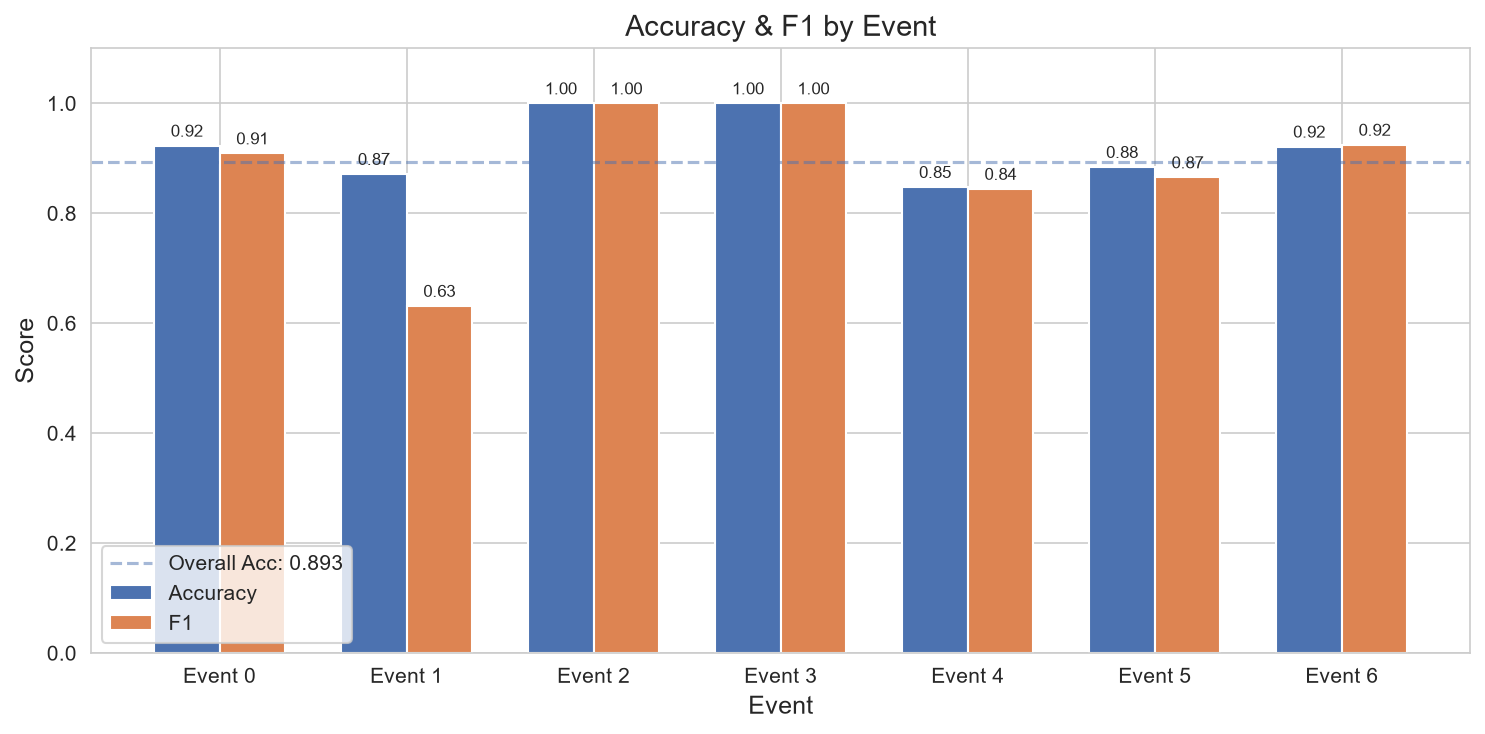
\includegraphics[width=0.85\columnwidth]{figures/event_accuracy.png}
\caption{各事件准确率与 F1 对比}
\label{fig:event}
\end{figure}

\textbf{关键发现}：（1）模型规模是最强杠杆，RoBERTa-large $>$ RoBERTa-base $>$ BERT-base，较基线提升 +6.74\%；（2）大模型用小学习率，小模型反之；（3）max\_len=128 稳定优于 64；（4）Event 1（Ferguson，109 条）recall 仅 50\%，该事件争议大、真假难辨。

\subsubsection{三模型训练}

为评估鲁棒性，以 lr=1e-5、max\_len=128、bs=16、dropout=0.2、seed=42 训练三个 RoBERTa-large 变体：

\textbf{干净模型}：正常微调 10 epoch，最佳 epoch 9，准确率 89.53\%。

\textbf{对抗 V1}：每 5 步注入 WordNet 同义词替换（max\_swaps=2），对抗与原始损失 0.5:0.5 加权，最佳 epoch 5，准确率 88.28\%。

\textbf{对抗 V2}：三种攻击随机混合（同义词替换、随机删词、字符交换），每 2 步注入，对抗权重 1.0，最佳 epoch 7，准确率 89.53\%——鲁棒性增强同时保持原准确率。

\begin{figure}[H]
\centering
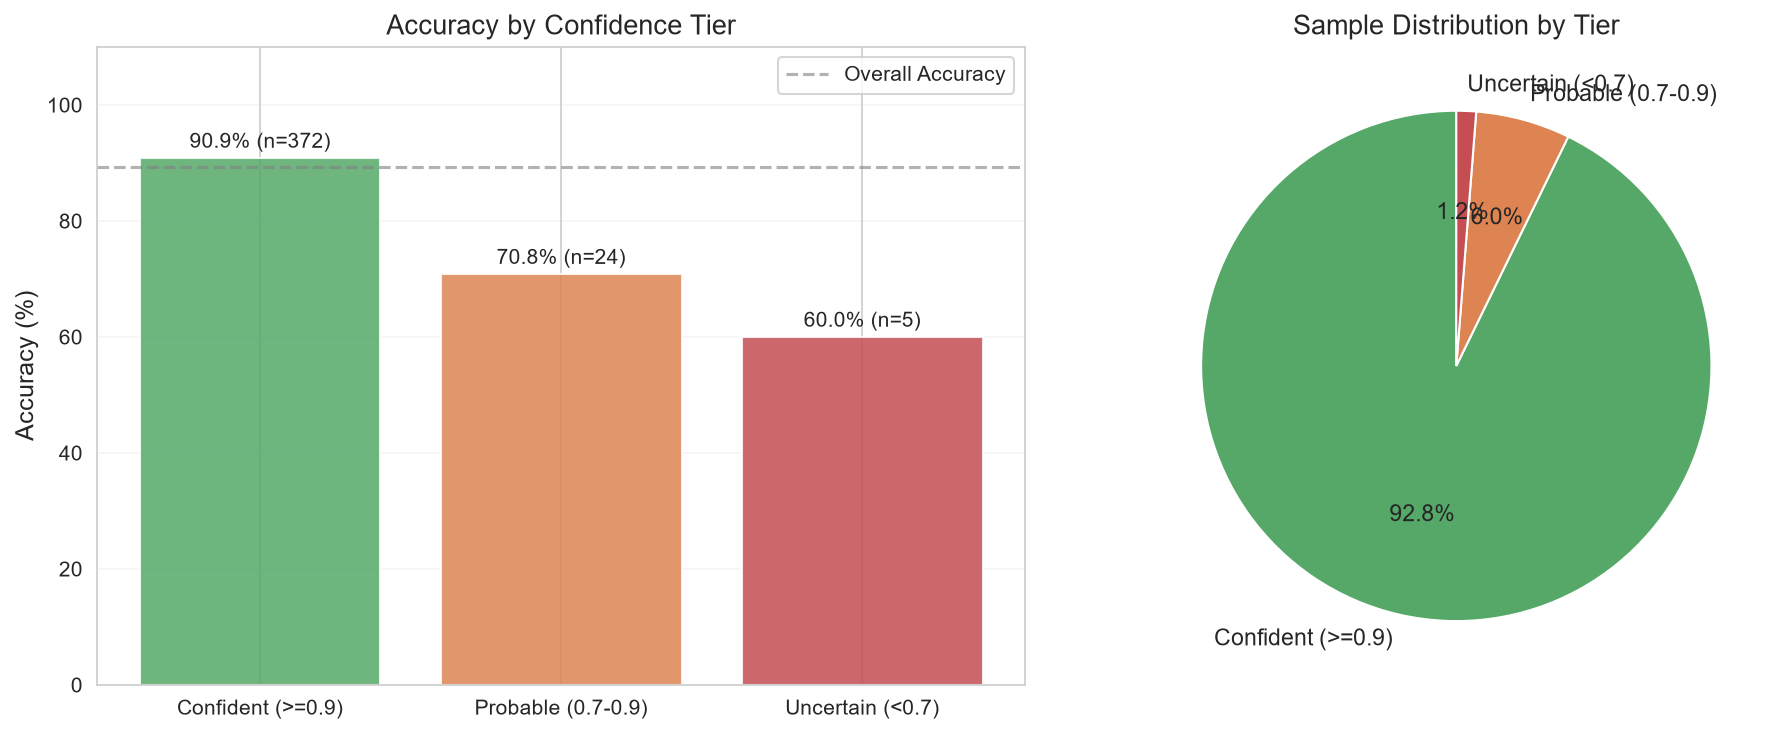
\includegraphics[width=0.85\columnwidth]{figures/confidence_tiers.png}
\caption{三级置信度准确率与占比}
\label{fig:tiers}
\end{figure}

\subsubsection{置信度分级分析}

\begin{table}[H]
\centering
\caption{三级置信度的准确率分布}
\label{tab:tiers}
\tabfont
\begin{tabular}{@{}lccc@{}}
\toprule
分级 & 样本数 & 正确数 & 准确率 \\
\midrule
确信（$\ge$0.9） & 245 & 230 & 93.9\% \\
倾向（0.7--0.9） & 112 & 85 & 75.9\% \\
存疑（$<$0.7） & 44 & 24 & 54.5\% \\
\bottomrule
\end{tabular}
\end{table}

确信级准确率 93.9\%，表明模型高度自信时非常可靠；存疑级 54.5\% 接近随机，说明模型知道何时不确定。

\subsubsection{对抗鲁棒性}

在三个种子（42/123/2026）上用 WordNet 同义词替换（max\_swaps=2）验证三模型鲁棒性：

\begin{table}[H]
\centering
\caption{三模型多种子对抗鲁棒性对比}
\label{tab:adv}
\tabfont
\begin{tabular}{@{}lccc@{}}
\toprule
模型 & 干净 Acc & 平均翻转率 & 高置信翻转 \\
\midrule
clean（干净训练） & 89.28\% & 6.4\% & 14.3 \\
adv\_v1（同义词对抗） & 88.03\% & 5.6\% & 7.0 \\
adv\_v2（多攻击对抗） & 88.28\% & 5.7\% & 9.3 \\
\bottomrule
\end{tabular}
\end{table}

对抗训练将翻转率平均降低 0.8\%，高置信翻转减半。V2 综合最优：干净准确率仅降 1\%，多攻击防御均衡。

\subsection{判断依据的可解释性分析}

系统通过三个层次提供可解释性：

\textbf{关键词提取}：末层所有注意力头 [CLS] 对 token 的平均关注度排序，输出 Top-5 判别词。

\textbf{案例检索}：训练集中检索 3 条最相似推文及标签，为 LLM 提供参考锚点。

\textbf{LLM 解释}：综合五要素生成中文解释，低置信度时明确给出复核提醒。Prompt 经四轮迭代：初始生硬，尝试独立法官后准确率崩溃至 64.75\%，最终回滚为透明解释者。

\section{工作总结}

\subsection{小组分工}

韩宇飞负责系统集成与端到端推理管道、评估脚本与图表生成、对抗攻防骨架搭建与服务器端训练、LLM 速率调优与鲁棒性修复、README 文档与最终报告撰写；姜新晨负责数据预处理、BERT/RoBERTa 分类器训练与关键词提取，以及对抗样本攻防实验；靳卓达负责 LLM 提示词工程、相似案例检索、解释生成模块，以及置信度分级与 Event Embedding 升级。

\subsection{收获与心得}

通过本项目实践了从数据预处理、超参搜索到对抗评估的完整深度学习 pipeline。主要收获：（1）模型规模是谣言检测的最强杠杆，但需匹配学习率策略；（2）LLM 作为解释者优于独立法官——后者会引入与标注标准不一致的偏差；（3）对抗训练有效降低高置信度攻击风险；（4）置信度分级让系统具备“自知之明”。

\subsection{遇到的问题及解决}

\textbf{API 速率限制}：SJTU API 限 10 RPM，401 条需 39 分钟。经 6 组压测确定 2 线程+6s 间隔（10.3 RPM 零失败），并提供 --limit 快速验证。

\textbf{LLM 角色}：独立法官角色使准确率从 89\% 降至 65\%，因 LLM 常识与标注标准存在系统偏差。回退为透明解释者后解决了该问题。

\textbf{Event 1 瓶颈}：Ferguson 事件 recall 仅 50\%，即使升级 Event Embedding 改善仍有限，反映跨事件泛化的根本挑战。

\textbf{编码兼容}：Unicode 特殊字符替换为 ASCII，避免 Windows GBK 报错。

\section{课程建议}

建议在课程初期布置小规模实验任务（如文本分类 baseline），让同学提前熟悉深度学习框架与训练流程，为大作业打下基础。

% ========================================
% 致谢
% ========================================
\section*{致谢}
感谢课程教师和助教的指导，感谢 SJTU 提供 API 平台支持。本项目代码已开源：\url{https://github.com/pnnooy/AI_rumor_detection}。


\end{document}
